\documentclass[twocolumn]{article}
\usepackage[width=17cm,height=22cm]{geometry}
\usepackage[english]{babel}
\usepackage[utf8]{inputenc}
\usepackage{fancyvrb}
\usepackage{authblk}
\usepackage{hyperref}
\usepackage{outlines}
\usepackage{graphicx}
\usepackage{color}
\DeclareGraphicsExtensions{.pdf,.png,.jpg}

\definecolor{vthierry}{RGB}{80,0,120}\newcommand{\vthierry}[1]{{\color{vthierry}{#1}}}
\definecolor{thalita}{RGB}{51, 153, 255}\newcommand{\thalita}[1]{{\color{thalita}{#1}}}


\bibliographystyle{alpha}
\title{From shortcuts to architecture optimization in deep-learning}
\author[1]{Thalita F. Drumond}
\author[1]{Thierry Vi\'eville}
\author[1]{Fr\'ed\'eric Alexandre}
\affil[1]{Mnemosyne team, INRIA Bordeaux}
\begin{document}
\maketitle

\begin{abstract}
  bla bla.
\end{abstract}
\medskip

\noindent\textbf{Keywords}: Deep-learning, Meta learning, Representation learning.

\section*{Introduction}

What is called structured hierarchical deep machine learning \cite{Deng2013Deep}, say deep-learning, uses ``a cascade of many layers of nonlinear processing units for feature extraction and transformation, each successive layer using the output from the previous layer as input''. Regarding visual tasks such as object recognition, categorization or segmentation, higher level features are derived from lower level features to form a hierarchical representation, with different levels of abstraction. Then, upper (i.e., shallower) fully connected layers often complete the functional transformation, before a readout layer (e.g., a softmax or support-vector machine for task categorization) \cite{Srinivas2016Taxonomy}. Starting with LeNet-5 \cite{Lecun1998Gradient}, different successful solutions have been evaluated on large data-base benchmarks (e.g., AlexNet\cite{Krizhevsky2012Imagenet}, ZF net \cite{Zeiler2014Visualizing}, Overfeat \cite{Sermanet2013Overfeat}, VGG \cite{Simonyan2015Very},  GoogLeNet \cite{Szegedy2014Going}, residual nets \cite{He2016Deep}). For all of them the architecture is given a priori, based on qualitative general considerations.

Such classical deep-learning architecture is most often a pipe-line of layers, as in VGG networks \cite{Simonyan2015Very}, which is going to be considered as a baseline in our study, the authors proposing several variant in terms of number of layers. Beyond a simple sequence of layers, it has been observed that shortcuts can strongly improve the performance thanks to what is called residual-learning \cite{He2016Deep}. Moreover, several deep-learning architectures combine parallel layers, such as segmentation using super pixel computation \cite{Farabet2013Learning}, combination on several parallel layers in \cite{Szegedy2014Going}, or final layer combination of intermediate layers (ex. skip-pooling in \cite{Shelhamer2016Fully}). These are suitable choices proposed by experiment scientist based on their human experience. 

\vthierry{
In many works, different variations of the same architecture (ZF net \cite{Zeiler2014Visualizing},  VGG \cite{Simonyan2015Very} , residual nets \cite{He2016Deep}, Inception-v3,-v4,-residual \cite{Szegedy2016Inception}) are compared or compare with their predecessor (e.g., residual net compared to plain VGG). It is also common to compare with other architectures focused on the same task. For instance, semantic segmentation works usually compare to Fully Convolutional nets \cite{Shelhamer2016Fully}, Segnet \cite{Badrinarayanan2015Segnet}, dilated conv nets\cite{Yu2016Multi}. Such manual and one shot comparisons are mandatory to validate a method, but do not demonstrate that one or another method is better on any future data set.

A step further, it has been proposed to use machine learning to explore a neural network architecture. The way to automate the design of machine learning models, is to consider meta-learning, i.e., to train a child network a get an accuracy in order a meta-adjustment to adjust the architecture itself, using e.g. evolutionary algorithms \cite{Real2017Large} and reinforcement learning \cite{Zoph2016Neural}. In this latter study, the machine-chosen architecture did incorporate unusual multiplicative combinations, present in LSTM units, as used for instance in scene labeling \cite{Byeon2015Scene}, beyond usual manual choices. \thalita{@TV soit regarder plus de refs sur le meta-learning}. 
% Reprendre les refs de sholarpedia et de Zopf, voir notion de perplexity
However, these methods are rather heavy, and as pointed out by their authors, are more a way to explore different architectures, than to generate an optimized architecture given a data set. As an alternative, we would like to explore how we could generalize usual parameter optimization to architecture optimization. \thalita{@TFB voir un meilleur argument ?}
}

Could it thus be possible to go a step further and, within the network adjustment itself, not only learn the layer parameters, i.e., the weights, but also learn how to adjust both the number of layers and the meta-parameters of a given layer ? Could we also not only consider a sequence of layers, but a more general acyclic graph of layers ? 

This is the double problem we want to tackle here. The key-point is that we want to have this structural optimization, not as a meta-parameter combinatory adjustment, but considering continuous parameters adjusted with the layer parameters.

In the next {\em methods} section we introduce a heuristic allowing us to not only adjust the deep-learning parameters but also some on the architecture meta-parameters and connections. In the {\em results} section we start experimenting such mechanism to evaluate the feasibility of these new ideas. In the final {\em conclusion} we discuss the improvements we can expect from such an innovative learning method.

\section*{Methods}

We are going to implement this general idea of adjusting a deep-learning architecture and related parameters using five ingredients.

\paragraph*{From layer sequence to acyclic graph.}

On one hand, considering a deep-learning layer sequence, we are going to combine each layer output with shortcuts from all deeper layers.  This allows us to define an acyclic graph with the output as supremum and the input as infimum. Restraining shortcuts direction from shallower to deeper layer guarantees the generation of an acyclic graph, i.e., without any recurrent link. On the reverse, any acyclic graph can obviously be defined in this framework, where the index of the layer corresponds to a so-called topological ordering of the graph (as defined, e.g by the Kahn's algorithm here simplified since we have a unique start node). This means that for $L$ layers we generate $L \, (L-1)/2$ new links, with one common modulatory weight for all units of a layer, thus one weight on each link. Please note that we do not consider a lattice here but any acyclic graph with a infimum and supremum, as illustrated in Fig.\ref{acyclicgraph}.

\begin{figure}
\centering
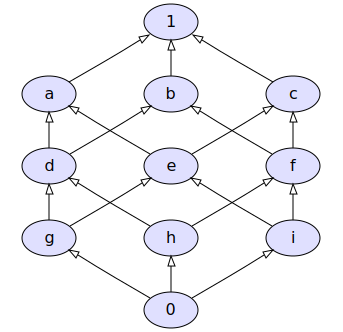
\includegraphics[width=0.3\textwidth]{img/acyclicgraph}
\caption{An example of deep acyclic architecture, combining several parallel computations, with input layer labeled $0$ and the output layer labeled $1$. This is not a lattice. Reproduced from \href{https://en.wikipedia.org/wiki/Lattice\_\%28order\%29\#/media/File:Pow3nonlattice.svg}{Wikipedia}.}
\label{acyclicgraph}
\end{figure}

Given a set of layers, the proposed method does not always generate all possible acyclic graphs, because a fixed initial total ordering of the layers is considered, which is not modified by the added shortcuts. If layers are uniform, i.e., if what is performed by one layer could be equally performed by another, providing the weights are transferred, then it is not a limitation (layers are interchangeable). Otherwise, only a reasonable subset of possible acyclic graphs is explored.

\paragraph*{Output sparse linear combination.}

If we write $x_{{\bf p}, l}(t)$ the activity at time $t$ of the $l$-th layer at the location ${\bf p}$ on the layer (e.g., ${\bf p}$ is a 2D location for a retinotopic coordinate when processing an image), and ${\bf x}_l = {\bf f}_l\left({\bf x}_{l-1}\right)$ the transform from on layer to another, the proposal is to now consider: $${\bf x}_l = w_{ll} \, {\bf f}_l\left({\bf x}_{l-1}\right) + \sum_{k < l} w_{lk} \, {\bf x}_k,$$ adding $L\,(L-1)/2$ modulatory parameters $w_{lk}$ with $k < l$, constraining $\sum_{k \leq l} w_{kl} = 1$ to avoid parameter redundancy. 
The design choice is to make a global ``soft-switch'' between layers and/or short cut (and not to combine each value between layers separately). By ``switch'', we mean that we target sparse estimation, i.e. to set a maximal number modulatory parameters to zero.
To this end, given an original criterion, ${\cal C}$, we propose to minimize: $${\cal C} + \sum_{l,k<l} |\tilde{w}_{kl}|,$$ thus a ${\cal L}_1$ criterion, with: $\tilde{w}_{ll} = 1 - \sum_{k < l} |\tilde{w}_{lk}|$.

We then define: $$w_{kl} = H(|\tilde{w}_{kl}| - w_{thres})\, \tilde{w}_{kl}, k \leq l$$  where $H(u)$ is the Heaviside function, in order to threshold the obtained values, assuming these values to be separated in two sets of (i) negligible an (ii) non negligible values. 

A natural choice is to set: $$\begin{array}{rcll} w_{thres} &=& \mbox{arg max}_{w_\bullet} & \min_{w_\bullet < |w_{kl}|}(|w_{kl}|) - \\ &&& \max_{|w_{kl}|> w_\bullet}(|w_{kl}|),\\ \end{array}$$ the threshold being chosen to maximize the difference between values higher and lower than the threshold. Such threshold is very simply computed at each step, by sorting the obtained $w_{lk}$ values, including $w_{ll}$, in increasing order and selecting the threshold where the difference between two values is maximal.

\paragraph*{Considering different layer variants.}

A step further, we may consider several convolution mask (e.g., a $5 \times 5$ mask size versus $3 \times 3$ or $1 \times 1$) for a given resolution. In VGG, authors note that stacking several $3 \times 3$ convolution layers has an effective receptive field of $5 \times 5$ (for two layers) or more. The resulting process is however not equivalent in terms of non-linearity, while the number of parameters is not the same. Here, the proposal is to also adjust the convolution mask size. 

\begin{figure}
\centering
\includegraphics[width=0.5\textwidth]{img/layer-variants}
\caption{The configuration to connect three layer variants (here different convolution mask size) to the related soft-switch.}
\label{layer-variants}
\end{figure}

To this end, we introduce in the layer sequence, three layers with the same meta-parameters but different convolution mask sizes, the higher mask size being, say, in the deeper position. We then rely on the previous sparse linear combination to switch between these alternatives, using two variants
\\- Not all connections are considered but only those corresponding to a connection of the variants as schematized in Fig.~\ref{layer-variants}, and we write $${\bf x}_l = \sum_{l'} w_{l'l} \, {\bf f}_{l'}\left({\bf x}_{l-1}\right) + \sum_{k < l} w_{lk} \, {\bf x}_k,$$ where $l' \in \{1, 2, 3\}$ indexes the layer variants.
\\ - The previous soft-switch is reused still minimizing a sparse ${\cal L}_1$ criterion but now thresholding $w_{l'l}$ in order to have only one non-zero value\footnote{Formally the equations now write: $$\begin{array}{rcl}
w_{kl} &=& H(|\tilde{w}_{kl}| - w_{thres})\, \tilde{w}_{kl}, k < l\\
w_{l'l} &=& H(|\tilde{w}_{l'l}| - \max(|\tilde{w}_{l'l}|) + \epsilon)\, \tilde{w}_{l'l},\\
\end{array}$$ for some small $\epsilon$.}, while the $w_{kl}$ and $w_{l'l}$ are thresholded as specified previously.

The proposed method is not limited to the convolution mask size only. We could have considered different non-linearity profiles (e.g., a sigmoid, versus a ReLU). However  it seems well established \cite{Glorot2010Understanding}, in this application fields, that ReLU (i.e., $f(u) = H(u) \, u$, i.e., a rectification) is a better choice. We also could have considered complementary tools such as Local Response Normalisation, but it has already be verified that it does not significantly improve the performances \cite{Simonyan2015Very}. A step further, separable convolutions kernels (thus with $2\,w$ parameters instead of $w^2$, for a $w \times w$ mask size) have been considered, with interesting performances \cite{Chollet2016Xception}. In this preliminary study, we only consider non-separable masks, but the method is straightforward to generalize to other layer variants.

\paragraph*{Connecting the different layers.}

With the proposed heuristic, layers with different resolution and number of channels are connected. Let us discuss how to perform such connections.

If we assume that along the initial layer sequence, (i) layer resolution decreases, and the (ii) number of channel increases, while higher resolution and higher number of channels is always a multiple of a lower one, then the shortcut connections are obvious to define by e.g., max-pooling to connect a higher resolution to a lower one, and, e.g., demultiplexing by connecting each channel of the deeper layer to a uniform number of channels in the present layer.

Common deep-learning architectures combine deeper convolution layers, with shallower fully connected layers, these latter layers being adapted to a given task. In particular, in VGG it is proposed to use a few layers at different resolutions. Such shallower layers may be considered as a ``one'' channel layer, with a convolution mask size equal to the layer size. In other words, the previous connection mechanisms applies to both kind of layers.

With the present heuristic it is expected that some layers are going to be ``disconnected'': This happens if $w_{ll} = 0$, i.e., if it is numerically preferable not to use the layer output but deeper layers value. This is an interesting property since it allows the estimation to also minimize the number of layers. This also happens when comparing different layer variants. This property has however two consequences: On one hand, it must be detected by the code in order not to further optimize useless weights. On the other hand, this means that we implicitly start with a ``maximal'' architecture with all possible layers, and decimate some of them. 

Such design has a limit and we would like to further integrate another mechanism.

\paragraph*{Re-generating the deep-learning architecture.}

The proposed adjustment has some limit. If the estimation result is that all layers are indeed useful to obtain an optimal, what about a bigger architecture ? For instance, with even more layers and even more channels ? On the other hand, if we compare, say $3 \times 3$, $5 \times 5$ convolution mask sizes and obtain that the latter performance is better, what about testing the $7 \times 7$ size ? In other words, the combinatory of the problem is too large to start with a huge architecture integrating all possibilities.

Our framework must be extended with the possibility to automatically regenerate a different deep-learning architecture with all weights initialized from the previous one, by copy or up/down sampling. In order to automatize this step, we propose to encode a given architecture\footnote{Such an architecture code may write:
\\-1 A convolution writes $C(s,w,c)$ with $w^2\,c$ weights:
\\-1.1 for an image size $2^s \times 2^s, s \in \{9, 8, 7, 6, 5, 4\}$,
\\-1.2 using a convolution mask size of $(1+2\,w)\times (1+2\,w), w \in \{0, 1, 2, 3\}$,
\\-1.3 and outputing $2^c, c \in \{6, 7, 8, 9\}$ channels.
\\-2 A fully connected layer writes $F(n)$ ,
\\ 2.1 where $2^n, n \in \{10, 11, 12\}$ is the number of units,
\\ while the shallowest layer is a soft-max writes $S()$, e.g.:
\begin{center}{\scriptsize  
C(8,1,6),C(8,1,6),C(7,1,7),C(7,1,7),C(6,1,8),C(6,1,8),\\
C(5,1,9),C(5,1,9),C(4,1,9),C(4,1,9),F(12),F(12),F(10),S()}
\end{center}
for the B configuration of the VGG networks \cite{Simonyan2015Very}.}, and to use this code to derive the next architecture when an architecture has been validated.

\vthierry{
  NE PAS PRENDRE EN COMPTE CE QUI SUIS :)

We are going to rely on the following rules:
\\- In valid deep-learning sequences the image size can not increase, and the number of channels can not decrease, while the number units in fully connected layer can not increase.
\\- Regarding layer variants, where three variants are evaluated, if the optimal value is not the middle one, a new triplet of value (if not at the layer variant bound) is to be generated.
\\- If in an initial architecture has not be reduced after learning, then it is worthwhile to increase the depth, adding new layers. \
\\- All tested layers are registered, in order not to regenerate an already evaluated layer.
}

\vthierry{Et c est la que je sajs pas du tout comment continuer :) mais je regarde !}

\section*{Results}

\vthierry{Here we thus propose to simply:
\\- randomly draw the relative proportion of learning and test samples between 0\% and 100\% from a truncated Gaussian distribution, of mean 50\% and standard-deviation 16\% (in order to fit in the [0\%,100\%] interval with $P>0.99$).
\\- randomly separate samples between both learning set and test set
\\- performing the estimation and evaluate the result on the test set
\\- update the parameters if and only if the test set performance improves ... [OU PAS : JUSTE UNE BASE DE DICUSSION]}

\section*{Conclusion}

The present process allows to explore several properties of a given deep architecture. 
\begin{enumerate}
\item How many layers at a given resolution and for a given processing step ?
\item How the resolution evolves along the deep-learning sequence ?
\item What is the best channel expansion from one layer to another ?
\item What is the best resolution mask at a given processing level ?
\item Should residual learning (i.e., learn only a weighted difference between two layers output, instead of the layer value only) ?
\item Could combination of parallel processing instead of sequential one be a better option at a given processing level ?
\end{enumerate}

\bibliography{thalita.bib}

\end{document}
